\documentclass[a4paper,12pt]{article}

\usepackage{mystyle}

\graphicspath{ {images/} }

\definecolor{my-red}{RGB}{248, 23, 134}
\definecolor{my-blue}{RGB}{5, 91, 206}
\definecolor{my-grey}{RGB}{128,128,128}


\author{Алексеев Василий}


\title{Семинар 9}
\date{10 ноября 2022}


\begin{document}
  \maketitle
  
  \tableofcontents

  \thispagestyle{empty}
  
  \newpage
  
  \pagenumbering{arabic}


  \section{Поверхности второго порядка}
  
  Любую поверхность второго порядка, как и кривую второго порядка на плоскости, можно задать в некоторой общей декартовой системе координат уравнением второй степени от координат точки.
  Но в случае поверхностей переменных в уравнении будет три: $x$, $y$ и $z$.
  
  Так же, как и для кривой второго порядка на плоскости, общее уравнение поверхности второго порядка с помощью ряда замен переменных можно привести к одному из нескольких канонических видов.  % TODO: check Bec
  Более того, некоторые поверхности второго порядка можно получить вращением вокруг оси симметрии соответствующей кривой второго порядка.
  
  Далее в основном рассмотрим некоторые из таких поверхностей вращения.
  
  
  \subsection{Эллипсоид}
  
  Пусть на плоскости в прямоугольной декартовой системе координат $OXZ$ эллипс задан уравнением:
  \[
    \frac{x^2}{a^2} + \frac{z^2}{c^2} = 1
  \]
  
  Перейдём в пространство.
  Выберем в пространстве прямоугольную декартову систему координат $OXYZ$ (пусть ось $OY$ проведена, например, так, чтобы система координат в пространстве была правой).
  И будем вращать указанный ранее эллипс вокруг оси $OZ$ (\ref{fig:ellipse-rotate-1}).
  
  \begin{figure}[h]
    \centering

    \includegraphics[width=0.8\textwidth]{ellipse-rotate-1}
  
    \caption{Вращение эллипса вокруг оси $OZ$.}
    \label{fig:ellipse-rotate-1}
  \end{figure}
  
  Все точки эллипса будут вращаться по окружностям, ``нанизанным'' на ось $OZ$.
  Рассмотрим точку $M_0(x_0, 0, z_0)$ эллипса.
  При вращении она в какой-то момент ``перейдёт'' в точку $M$ с координатами $(x, y, z)$.
  Точки $M_0$ и $M$, очевидно, лежат на одной и той же плоскости, перпендикулярной оси $OZ$, то есть $z \hm= z_0$.
  Расстояние до оси вращения как от точки $M_0$, так и от точки $M$, одинаково:
  \[
    \sqrt{x_0^2 + 0^2} = \sqrt{x^2 + y^2}
  \]
  
  При этом точка $M_0$ лежит на эллипсе:
  \[
    \frac{x_0^2}{a^2} + \frac{z_0^2}{c^2} = 1
  \]
  
  Если мы теперь заменим $x_0^2$ в равенстве выше на $x^2 \hm+ y^2$, то получим \emph{уравнение эллипса, образованного при вращении точки $M_0$ вокруг оси $OZ$} (координаты $x$, $y$~---~координаты \emph{некоторой} точки):
  \[
    \frac{x^2 + y^2}{a^2} + \frac{z_0^2}{c^2} = 1
  \]
  
  Для получения уравнения эллипсоида (соотношения от координат $x$, $y$, $z$) надо теперь ещё ``заменить'' $z_0^2$ на $z^2$ (чтобы координата $z$ тоже могла ``варьироваться''):
  \[
    \frac{x^2 + y^2}{a^2} + \frac{z^2}{c^2} = 1
  \]
  
  Итак, каждая точка эллипса при вращении будет двигаться по окружности.
  Уравнению выше удовлетворяет \emph{любая} точка \emph{любой} такой окружности~---~траектории вращения точки эллипса.
  По построению, только из таких точек и состоит описанный эллипсоид.
  Другие точки, не с окружностей, уравнению не удовлетворяют.
  Поэтому полученное уравнение~---~уравнение эллипсоида.
  
  Если дополнительно провести сжатие вдоль оси $OY$\footnote{Здесь имеется в виду не сжатие самой оси $OY$ системы координат $OXYZ$. Ведь если система координат $OXYZ$ была прямоугольной, то сжимать её ось будет, скорее всего, ``не очень хорошо''. Имеется в виду именно сжатие эллипсоида вдоль оси $OY$: каждая точка $(x, y, z)$ исходного эллипсоида переходит в точку $(x, ky, z)$, где $k \hm> 0$ (например, $k \hm= a \hm/ b$, $b \hm> 0$).}, то можно прийти к общему уравнению эллипсоида:
  \begin{equation}
    \label{eq:ellipsoid}
    \boxed{
      \frac{x^2}{a^2} + \frac{y^2}{b^2} + \frac{z^2}{c^2} = 1
    }
  \end{equation}
  
  \begin{figure}[h]
    \centering

    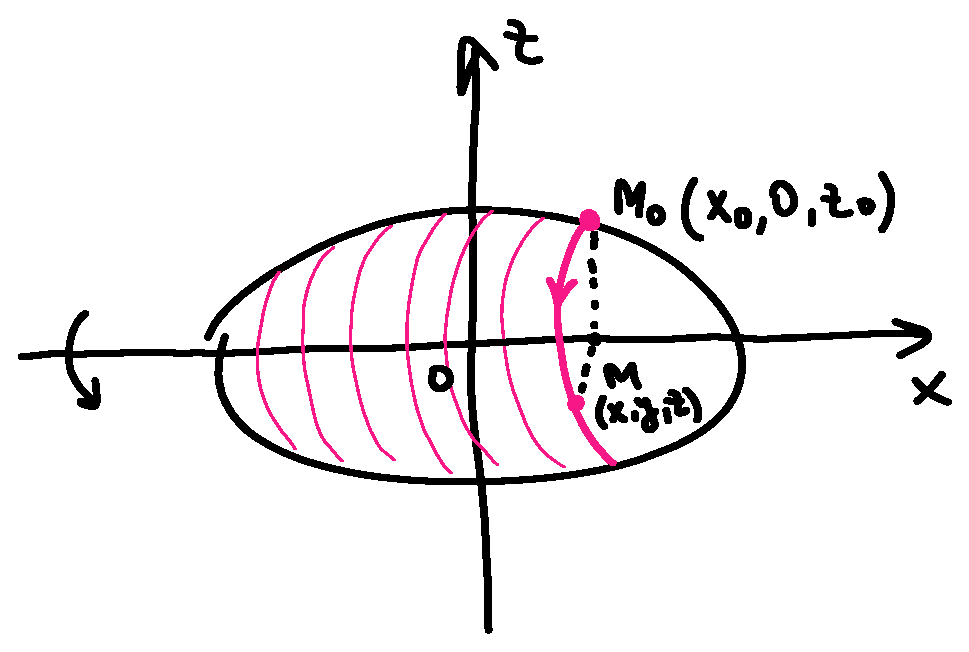
\includegraphics[width=0.8\textwidth]{ellipse-rotate-2}
  
    \caption{Вращение эллипса вокруг оси $OX$.}
    \label{fig:ellipse-rotate-2}
  \end{figure}
  
  Если исходный эллипс вращать вокруг оси $OX$, а не $OZ$ (\ref{fig:ellipse-rotate-2}), то эллипсоид получится другой:
  \[
    \frac{x^2}{a^2} + \frac{z^2 + y^2}{c^2} = 1
  \]
  но после сжатия вдоль $OY$ его уравнение всё равно будет вида~(\ref{eq:ellipsoid}).
  
  
  \subsection{Гиперболоид}
  
  \subsubsection{Однополостный}
  
  Теперь рассмотрим гиперболу в её канонической системе координат и будем вращать её вокруг какой-нибудь оси симметрии.
  Пусть гипербола задана в плоскости $XOZ$ уравнением:
  \[
    \frac{x^2}{a^2} - \frac{z^2}{c^2} = 1
  \]
  
  \begin{figure}[h]
    \centering

    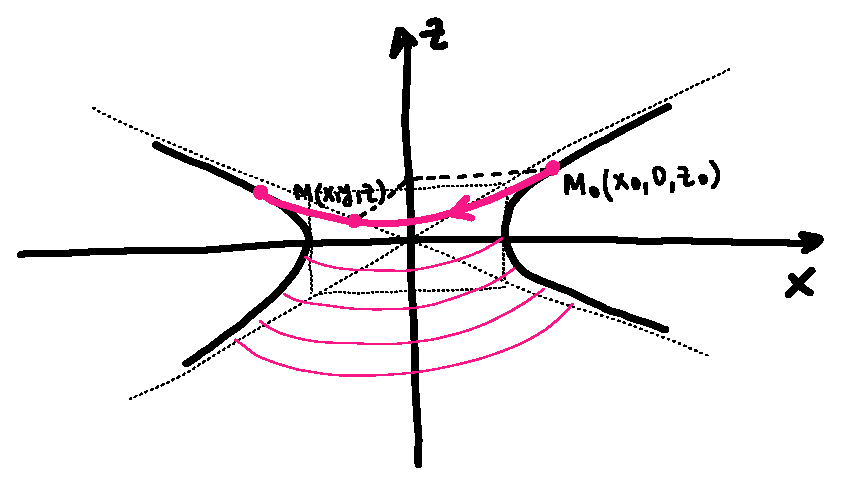
\includegraphics[width=0.8\textwidth]{hyperbola-rotate-1}
  
    \caption{Вращение гиперболы вокруг оси $OZ$.}
    \label{fig:hyperbola-rotate-1}
  \end{figure}
  
  Если вращать её вокруг оси $OZ$ (\ref{fig:hyperbola-rotate-1}), то, по аналогии с эллипсом и эллипсоидом, получаем:
  \[
    \frac{x^2 + y^2}{a^2} - \frac{z^2}{c^2} = 1
  \]
  
  И после сжатия вдоль оси $OY$:
  \begin{equation}
    \label{eq:hyperboloid1}
    \boxed{
      \frac{x^2}{a^2} + \frac{y^2}{b^2} - \frac{z^2}{c^2} = 1
    }
  \end{equation}
  
  Полученная поверхность, которую в некоторой прямоугольной декартовой системе координат можно описать уравнением вида (\ref{eq:hyperboloid1}), называется \emph{однополостным гиперболоидом} (``однополостным''~---~потому что одна полость посередине, ``гиперболоидом''~---~потому что получен вращением гиперболы).
  
  Но у гиперболы, как и у эллипса (отличного от окружности), две оси симметрии.
  И можно бы было вращать гиперболу вокруг оси $OX$ (\ref{fig:hyperbola-rotate-2})...
  
  
  \subsubsection{Двуполостный}
  
  \begin{figure}[h]
    \centering

    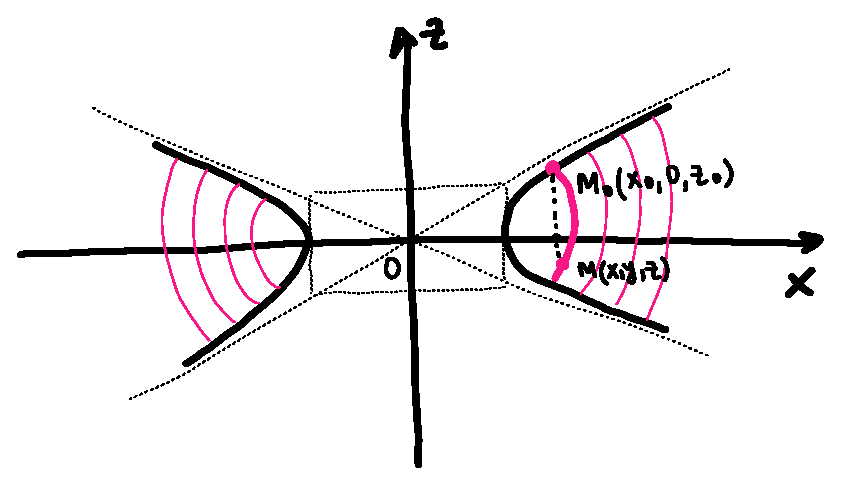
\includegraphics[width=0.8\textwidth]{hyperbola-rotate-2}
  
    \caption{Вращение гиперболы вокруг оси $OX$.}
    \label{fig:hyperbola-rotate-2}
  \end{figure}
  
  ...В таком случае уравнение поверхности вращения получилось бы таким:
  \[
    \frac{x^2}{a^2} - \frac{y^2 + z^2}{c^2} = 1
  \]
  
  И после сжатия, опять вдоль оси $OY$:
  \begin{equation}
    \label{eq:hyperboloid2}
    \boxed{
      \frac{x^2}{a^2} - \frac{y^2}{b^2} - \frac{z^2}{c^2} = 1
    }
  \end{equation}
  
  Полученная поверхность вращения называется \emph{двуполостным гиперболоидом} (потому что уже две полости).
  
  
  \subsection{Параболоид}
  
  \subsubsection{Эллиптический}
  
  Перейдём в вращению параболы вокруг оси симметрии.
  Пусть парабола задана в канонической системе координат уравнением
  \[
    x^2 = 2pz
  \]
  
  При вращении вокруг оси $OZ$ (\ref{fig:parabola-rotate-1}) получим поверхность
  \[
    x^2 + y^2 = 2pz
  \]
  
  \begin{figure}[h]
    \centering

    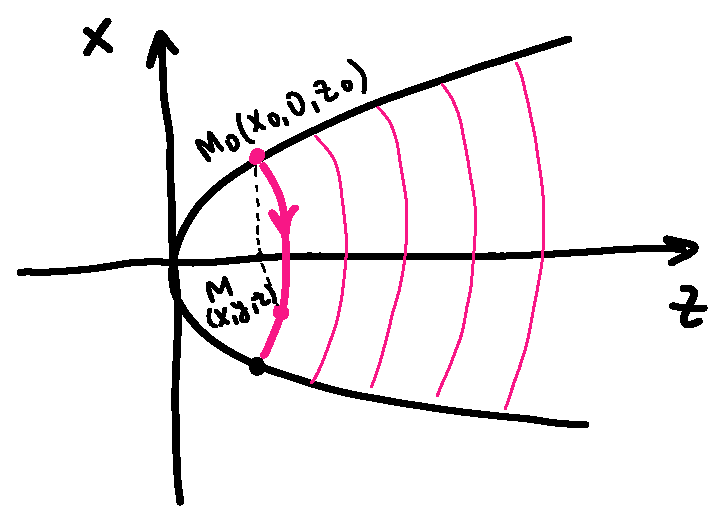
\includegraphics[width=0.5\textwidth]{parabola-rotate-1}
  
    \caption{Вращение параболы вокруг оси $OZ$.}
    \label{fig:parabola-rotate-1}
  \end{figure}
  
  Или, после сжатия-растяжения вдоль осей $OX$ и $OY$, можно прийти к уравнению вида:
  \begin{equation}
    \label{eq:paraboloid1}
    \boxed{
      \frac{x^2}{a^2} + \frac{y^2}{b^2} = 2z
    }
  \end{equation}
  
  Поверхность называется \emph{эллиптическим параболоидом} (``эллиптическим''~---~потому что в сечении плоскостями вида $z \hm= C$ получаются эллипсы).
  
  В полученном уравнении (\ref{eq:paraboloid1}) можно поменять знак с ``плюса'' на ``минус'', и тогда получится...
  
  
  \subsubsection{Гиперболический}
  
  ...следующее уравнение:
  \begin{equation}
    \label{eq:paraboloid2}
    \boxed{
      \frac{x^2}{a^2} - \frac{y^2}{b^2} = 2z
    }
  \end{equation}
  
  Поверхность, описываемая в некоторой декартовой прямоугольной системе координат уравнением (\ref{eq:paraboloid2}) называется \emph{гиперболическим параболоидом} (``гиперболическим''~---~потому что в сечении плоскостями вида $z \hm= C$ получаются гиперболы).
  
  Гиперболический параболоид~---~не поверхность вращения.
  
  Как же его нарисовать?
  
  При $y \hm= 0$ имеем $x^2 \hm/ a^2 \hm= 2z$.
  Это~---~парабола (в плоскости $y \hm= 0$).
  Назовём её параболой $\Pi_{y=0}$, или $\textcolor{my-red}{\Pi_1}$.
  
  При $x \hm= 0$ получаем $-y^2 \hm/ b^2 \hm= 2z$.
  Это тоже парабола.
  Назовём её $\Pi_{x=0}$, или $\textcolor{my-blue}{\Pi_2}$.
  
  Очевидно, вершины парабол $\textcolor{my-red}{\Pi_1}$ и $\textcolor{my-blue}{\Pi_2}$ совпадают.
  Оси обеих парабол идут вдоль оси $OZ$.
  Но парабола $\textcolor{my-red}{\Pi_1}$ направлена ``вверх'' по оси $OZ$.
  А парабола $\textcolor{my-blue}{\Pi_2}$ направлена ``вниз''.
  Ещё из интересного можно отметить, что параболы $\textcolor{my-red}{\Pi_1}$ и $\textcolor{my-blue}{\Pi_2}$ лежат в двух взаимно перпендикулярных плоскостях.
  
  ``Нарисуем'' обе параболы $\textcolor{my-red}{\Pi_1}$ и $\textcolor{my-blue}{\Pi_2}$ (см. рисунок~\ref{fig:parabola-kinda-rotate-2}).
  
  \begin{figure}[h]
    \centering

    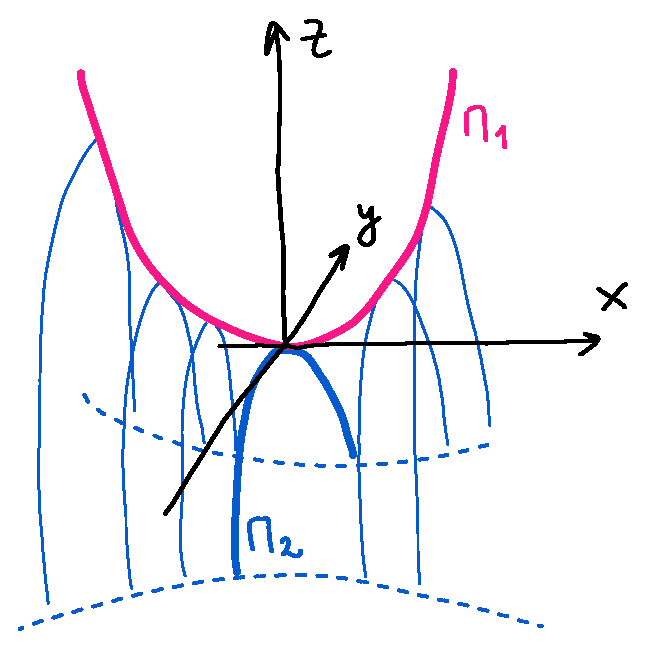
\includegraphics[width=0.8\textwidth]{parabola-kinda-rotate-2}
  
    \caption{Взгляд на гиперболический параболоид как на параболу, вершина которой ``скользит'' по другой параболе.}
    \label{fig:parabola-kinda-rotate-2}
  \end{figure}
  
  Далее, чтобы построить гиперболический параболоид, можно поступить следующим образом.
  Положим $x \hm= 1$.
  Сечение параболоида этой плоскостью описывается уравнением $-y^2 \hm/ b^2 \hm+ 1 \hm/ a^2 \hm= 2z$.
  Это парабола $\Pi_{x=1}$.
  Но при том же самом $x \hm= 1$ для параболы $\textcolor{my-red}{\Pi_1}$ имеем $1 \hm/ a^2 \hm= 2z$.
  Очевидно, вершина параболы $\Pi_{x=1}$ лежит на параболе $\textcolor{my-red}{\Pi_1}$ $(\Pi_{y=0})$.
  Парабола $\Pi_{x=1}$ как бы получается из параболы $\textcolor{my-blue}{\Pi_2}$ $(\Pi_{x=0})$ ``скольжением'' вдоль $\textcolor{my-red}{\Pi_1}$.
  Таким образом, на гиперболический параболоид можно смотреть как на поверхность второго порядка, полученную ``скольжением одной параболы по другой'' (\ref{fig:parabola-kinda-rotate-2}).
  Как на следующее семейство парабол, параметризуемых $x_0 \hm\in \RR$:
  \[
    \left\{
      \begin{aligned}
        &\left\{
          \begin{aligned}
            &-\frac{y^2}{b^2} + 2z_0 = 2z\quad \mbox{(``скользящая'' парабола, в данный момент напротив $x_0$)}\\
            &x = x_0
          \end{aligned}
        \right.\\
        &\frac{x_0^2}{a^2} = 2z_0\quad \mbox{(фиксированная парабола, по которой ``двигается'' вершина ``скользящей'')}\\
        &x_0 \in \RR\quad \mbox{(семейство ``скользящих'' парабол)}
      \end{aligned}
    \right.
  \]
  
  Можно бы было смотреть на параболоид немного по-другому.
  Положим $y \hm= 1$.
  В сечении параболоида этой плоскостью получаем кривую, описываемую уравнением $x^2 \hm/ a^2 \hm- 1 \hm/ b^2 \hm= 2z$.
  Следуя введённым обозначениям, эту параболу можно назвать $\Pi_{y=1}$.
  Но при $y \hm= 1$ для параболы $\textcolor{my-blue}{\Pi_2}$ имеем $-1 \hm/ b^2 \hm= 2z$.
  Таким образом, гиперболический параболоид может быть получен и как объединение ещё одного семейства парабол.
  Которые в этот раз скользят уже по параболе $\textcolor{my-blue}{\Pi_2}$:
  \[
    \left\{
      \begin{aligned}
        &\left\{
          \begin{aligned}
            &\frac{x^2}{a^2} + 2z_0 = 2z\quad \mbox{(``скользящая'' парабола, в данный момент напротив $y_0$)}\\
            &y = y_0
          \end{aligned}
        \right.\\
        &-\frac{y_0^2}{b^2} = 2z_0\quad \mbox{(фиксированная парабола, по которой ``двигается'' вершина ``скользящей'')}\\
        &y_0 \in \RR\quad \mbox{(семейство ``скользящих'' парабол)}
      \end{aligned}
    \right.
  \]
  
  \medskip
  
  Гиперболический параболоид построен.
  Теперь можно заметить ещё одно ``интересное''.
  Вспомним уравнение параболоида (\ref{eq:paraboloid2}):
  \[
    \frac{x^2}{a^2} - \frac{y^2}{b^2} = 2z
  \]
  
  Разобьём на множители левую и правую часть:
  \[
    \left(\frac{x}{a} - \frac{y}{b}\right) \left(\frac{x}{a} + \frac{y}{b}\right) = 1 \cdot 2z
  \]
  
  И составим такую систему (приравняв по одному множителю слева и справа):
  \[
    \left\{
      \begin{aligned}
        &\frac{x}{a} - \frac{y}{b} = 1\\
        &\frac{x}{a} + \frac{y}{b} = 2z
      \end{aligned}
    \right.
  \]
  
  Это пересечение двух плоскостей.
  То есть прямая.
  Но... из системы, задающей прямую, \emph{следует} уравнение параболоида (перемножив левые и правые части уравнений системы, получаем уравнение параболоида).
  Это значит, что прямая \emph{содержится} в гиперболическом параболоиде.
  Таким образом, описанная прямая~---~пример \emph{прямолинейной образующей} гиперболического параболоида.
  
  Но мы бы могли рассмотреть и такую систему:
  \[
    \boxed{
      \left\{
        \begin{aligned}
          &\alpha\left(\frac{x}{a} - \frac{y}{b}\right) = \beta \cdot 1\\
          &\beta\left(\frac{x}{a} + \frac{y}{b}\right) = \alpha \cdot 2z
        \end{aligned}
      \right.
    }
  \]
  при $\alpha^2 \hm+ \beta^2 \hm{\not=} 0$.
  Такая система тоже задаёт прямую, которая тоже целиком лежит на параболоиде.
  Получаем целое \emph{семейство прямолинейных образующих}.
  
  Если же мы теперь приравняем другие множители из уравнения параболоида, и снова ``подключим'' $\alpha$ и $\beta$, совместно не равные нулю, то получим ещё одно семейство прямолинейных образующих:
  \[
    \boxed{
      \left\{
        \begin{aligned}
          &\alpha\left(\frac{x}{a} - \frac{y}{b}\right) = \beta \cdot 2z\\
          &\beta\left(\frac{x}{a} + \frac{y}{b}\right) = \alpha \cdot 1
        \end{aligned}
      \right.
    }
  \]
  
  \medskip
  
  В случае \emph{однополостного гиперболоида}~(\ref{eq:hyperboloid1}) тоже можно бы было разложить левую и правую часть уравнения на множители (перенеся перед этим член с $y$ направо).
  И тоже можно бы было выписать две системы, задающие два семейства прямолинейных образующих.
  
  
  \section{Задачи}
  
  \subsection{\# 10.3(6)}
  
  Определить тип поверхности при разных $\lambda$:
  \[
    x^2 + \lambda (y^2 + z^2) = 1
  \]
  
  \begin{solution}
    Рассмотрим случай $\lambda \hm= 0$:
    \[
      x^2 = 1 \leftrightarrow \left[
        \begin{aligned}
          &x = -1\\
          &x = 1
        \end{aligned}
      \right.
    \]
    
    Получается две параллельных плоскости.
    
    \medskip
    
    Пусть теперь $\lambda \hm> 0$.
    Тогда можно считать $\lambda \hm= 1/p^2$, $p \hm> 0$:
    \[
      x^2 + \frac{y^2}{p^2} + \frac{z^2}{p^2} = 1
    \]
    
    Очевидно, это эллипсоид.
    Причём можно считать этот эллипсоид полученным в результате вращения эллипса $x^2 \hm+ z^2/p^2 \hm= 1$, $y \hm= 0$ вокруг оси $OX$. 
    
    \medskip
    
    Пусть теперь $\lambda \hm< 0$.
    В таком случае можно положить $\lambda \hm= -1/p^2$, $p \hm> 0$:
    \[
      x^2 - \frac{y^2}{p^2} - \frac{z^2}{p^2} = 1
    \]
    
    Это~---~двуполостный гиперболоид.
    Его можно бы было получить вращением гиперболы $x^2 \hm- z^2/p^2 \hm= 1$, $y \hm= 0$ вокруг оси $OX$.
  \end{solution}
  
  
  \subsection{\# 10.38 + 10.26}
  
  Составить уравнение прямого кругового цилиндра, проходящего через точку $M_0(1, 1, 2)$, и ось которого задана системой уравнений $l\colon x \hm= 1 \hm+ t$, $y \hm= 2 \hm+ t$, $z \hm= 3 \hm+ t$, $t \hm\in \RR$.
  
  \begin{solution}
    \vphantom{}
    
    \emph{Способ 1: ``излишне подробный''}.
    Очевидно, данных в задаче достаточно для задания цилиндра.
    И первым шагом хотелось бы найти его радиус...
    
    Направляющий вектор прямой~--~оси цилиндра $\bds a$ и начальная точка $A$ на оси цилиндра: $\bds a \hm= (1, 1, 1)$, $A(1, 2, 3)$.
    
    Из определения цилиндра следует, что в сечении кругового цилиндра плоскостями, параллельными основанию, будут получаться окружности.
    Каждой точке $M$ на поверхности цилиндра соответствует плоскость $\alpha$, перпендикулярная оси $l$ и при сечении цилиндра дающая окружность, на которой лежит эта точка.
    Общей же точкой для секущей плоскости $\alpha$ и оси цилиндра $l$ будет некоторая точка $P$ (см. рисунок~\ref{fig:cylinder-10-38})...
    
    \begin{figure}[h]
      \centering

      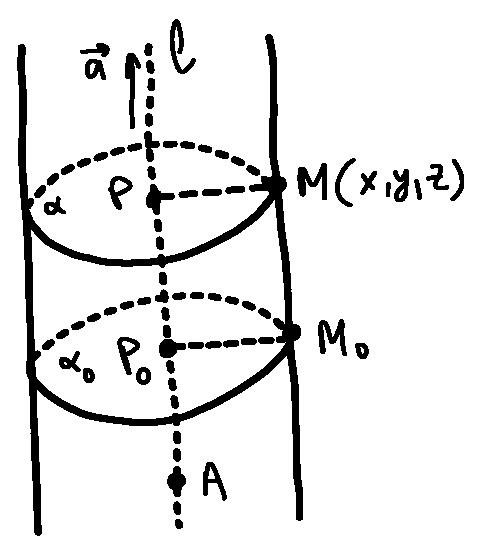
\includegraphics[width=0.45\textwidth]{cylinder-10-38}
    
      \caption{Точки цилиндра удалены от оси на одинаковое расстояние.}
      \label{fig:cylinder-10-38}
    \end{figure}
    
    Найдём точку $P_0$ на оси цилиндра, соответствующую точке $M_0$, данной в условии.
    Зная координаты точки $P_0$, можно будет найти радиус цилиндра как расстояние $\rho$ между точками $P_0$ и $M_0$: $R \hm= \rho(P_0, M_0)$.
    
    Направляющий вектор оси $\bds a$ является и вектором нормали плоскостей, перпендикулярных оси цилиндра.
    Поэтому всё семейство таких плоскостей, перпендикулярных оси, задаётся параметрическим уравнением
    \begin{equation}
      \label{eq:family-of-planes}
      x + y + z + D = 0,\quad D \in \RR
    \end{equation}
    
    Плоскость $\alpha_0$ для точки $M_0(1, 1, 2)$:
    \[
      1 + 1 + 2 + D_0 = 0 \Leftrightarrow D_0 = -4
    \]
    
    Пусть точке $P_0$ на оси соответствует значение параметра $t$, равное $\tau_0$.
    Тогда то, что $P_0$ лежит на той же плоскости, что и $M_0$, означает:
    \[
      (1 + \tau_0) + (2 + \tau_0) + (3 + \tau_0) - 4 = 0 \Leftrightarrow \tau_0 = \frac{-6 - (-4)}{3} = -\frac{2}{3}
    \]
    \[
      P_0\colon \left\{
        \begin{aligned}
          &x = 1 + \tau_0 = 1 - \frac{2}{3} = \frac{1}{3}\\
          &y = 2 + \tau_0 = 2 - \frac{2}{3} = 1\frac{1}{3}\\
          &z = 3 + \tau_0 = 3 - \frac{2}{3} = 2\frac{1}{3}
        \end{aligned}
      \right.
    \]
    
    И можно найти радиус цилиндра:
    \[
      R = \rho(P_0, M_0) = \ldots = \frac{\sqrt{6}}{3}
    \]
    
    Теперь рассмотрим некоторую точку $M(x, y, z)$ на цилиндре.
    Ей, как и точке $M_0$, соответствует некоторая плоскость $\alpha$ из семейства (\ref{eq:family-of-planes}) и точка $P$ на оси цилиндра.
    Пусть этой точке $P$ на оси соответствует значение параметра $t$, равное $\tau$.
    Тогда мы можем записать:
    \[
      \alpha\colon x + y + z + D = 0 \Leftrightarrow D = -(x + y + z)
    \]
    \begin{equation}
    \begin{split}
      P \in \alpha \Leftrightarrow (1 + \tau) + (2 + \tau) + (3 + \tau) + D = 0
      \Leftrightarrow \tau = \frac{-6 - D}{3}
    \end{split}
    \end{equation}
    
    Поэтому
    \begin{equation}
      \label{eq:t_P_prime}
      \tau = \frac{-6 + x + y + z}{3}
    \end{equation}
    
    И снова выписываем выражение для расстояния от точки $M$ (которая произвольная на цилиндре) до соответствующей ей точки $P$:
    \[
      \rho(M, P) = \sqrt{\bigl(x - (1 + \tau)\bigr)^2 + \bigl(y - (2 + \tau)\bigr)^2 + \bigl(z - (3 + \tau)\bigr)^2} = R
    \]
    
    Заменяя далее $\tau$ его представлением через координаты $x, y, z$ точки $M$ (\ref{eq:t_P_prime}), вспоминая найденный ранее $R$ и начиная ``варьировать координаты'' (далее $x$, $y$ и $z$ уже не фиксированные координаты некоторой случайно выбранной, но конкретной точки $M$, а ``координаты в уравнении'') получаем уравнение цилиндра:
    \[
      x^2 + y^2 + z^2 - xy - xz - yz + 3x - 3z + 2 = 0
    \]
    
    \medskip
    
    \emph{Способ 2: ``чересчур компактный''}.
    На самом деле для определения расстояния от точки $M$ до оси не обязательно было искать соответствующую точке $M$ точку $P$ на оси $l$.
    
    Пусть $\phi$~---~угол между векторами $\vv{AM}$ и $\bds a$.
    Тогда расстояние от $M$ до оси $l$ можно вычислить следующим образом:
    \[
      \rho(M, l) = |\vv{AM}| \sin\phi
        = \frac{\bigl|[\vv{AM}, \bds a]\bigr|}{|\bds a|}
    \]
    
    Точка лежит на цилиндрической поверхности в том и только в том случае, если она удалена от оси цилиндра на расстояние, равное радиусу.
    А радиус можно вычислить, используя данную в условии точку $M_0$.
    Итого:
    \[
      M \in \mbox{Цилиндр} \Leftrightarrow \rho(M, l) = R = \rho(M_0, l)
    \]
    \[
      \frac{\bigl|[\vv{AM}, \bds a]\bigr|}{|\bds a|} = \frac{\bigl|[\vv{AM_0}, \bds a]\bigr|}{|\bds a|}
    \]
    
    При этом:
    \[
      [\vv{AM}, \bds a] = \begin{vmatrix}
        \bds e_1 & \bds e_2 & \bds e_3\\
        x - 1    & y - 2    & z - 3\\
        1        & 1        & 1
      \end{vmatrix}
    \]
    \[
      [\vv{AM_0}, \bds a] = \begin{vmatrix}
        \bds e_1 & \bds e_2 & \bds e_3\\
        1 - 1    & 1 - 2    & 2 - 3\\
        1        & 1        & 1
      \end{vmatrix}
    \]
    
    И потому уравнение цилиндра (необходимое и достаточное условие на координаты точки $M$ для того, чтоб она лежала на цилиндре):
    \[
      (y - z + 1)^2 + (-x + z - 2)^2 + (x - y + 1)^2 = 0 + (-1)^2 + 1^2
    \]
    
    После упрощений:
    \[
      x^2 + y^2 + z^2 - xy - xz - yz + 3x - 3z + 2 = 0
    \]
  \end{solution}
  
  
  \subsection{\# 10.41}
  
  Найти уравнение и определить тип поверхности, образованной вращением прямой $l$, заданной уравнениями $x \hm= 0$, $y \hm- z \hm+ 1 \hm= 0$, вокруг оси $OZ$.
  
  \begin{solution}
    Что может получаться при вращении одной прямой вокруг другой?
    Если прямые параллельны, то будет цилиндр (см. предыдущий номер).
    Если пересекаются~---~конус (см. далее). % TODO: про конус
    Если скрещиваются, то... см. задачу 10.40.
    
    Проверим, как расположены друг относительно друга две данные в условии прямые.
    Но сначала найдём направляющий вектор $\bds a$ и начальную точку $\bds r_0$ вращаемой прямой $l$:
    \[
      \bds a = \left(\begin{vmatrix}0 & 0\\ 1 & -1\end{vmatrix}, \begin{vmatrix}0 & 1\\ -1 & 0\end{vmatrix}, \begin{vmatrix}1 & 0\\ 0 & 1\end{vmatrix}\right)
      = (0, 1, 1)
    \]
    \[
      \bds r_0 = (0, 0, 1)
    \]
    
    Поэтому прямую $l$ можно задать в виде системы скалярных параметрических уравнений так:
    \[
      \left\{
        \begin{aligned}
          &x = 0\\
          &y = t\\
          &z = 1 + t
        \end{aligned}
      \right.
    \]
    
    Направляющий вектор и начальная точка для оси $OZ$:
    \[
      \bds a_1 = (0, 0, 1),\ \bds r_1 = (0, 0, 1)
    \]
    
    Очевидно, что вращаемая прямая $l$ и ось вращения $OZ$ пересекаются в одной точке~---~в точке $(0, 0, 1)$.
    Поэтому поверхность вращения~---~конус.
    
    % TODO: pic
    Рассмотрим произвольную точку $M(x, y, z)$ на конусе.
    Этой точке соответствует точка $M_0(x_0, y_0, z_0)$, находящаяся на том же ``уровне'' по оси $OZ$, что и точка $M$, и лежащая на вращаемой прямой $l$.
    Расстояния от обеих точек до оси вращения одинаковы.
    Запишем же в виде формул перечисленные свойства:
    \[
      \left\{
        \begin{aligned}
          &z = z_0\\
          &x_0 = 0,\ y_0 = t_0,\ z_0 = 1 + t_0\\
          &\sqrt{x^2 + y^2} = \sqrt{x_0^2 + y_0^2}
        \end{aligned}
      \right.
    \]
    
    Откуда, исключая из последнего уравнения ``нулевые'' координаты и оставляя только $x$, $y$ и $z$ некоторой точки $M$, получаем уравнение конуса (координаты $x$, $y$ и $z$ удовлетворяют уравнению в том и только в том случае, когда $M$ лежит на конусе):
    \[
      x^2 + y^2 - (z - 1)^2 = 0
    \]
  \end{solution}


  \subsection{\# 10.65(1)}
  
  Найти центр сечения эллипсоида
  $
    x^2 \hm+ 2y^2 \hm+ 4z^2 \hm= 40
  $
  плоскостью
  $
    x + y + 2z \hm= 5
  $.
  
  \begin{solution}
    Выразим $x$ из уравнения плоскости через $y$ и $z$ (то есть ``перейдём'' в секущую плоскость):
    \[
      x = 5 - y - 2z
    \]
    и подставим в уравнение эллипсоида, чтобы получить уравнение сечения:
    \[
      \left\{
        \begin{aligned}
          &(5 - y - 2z)^2 + 2y^2 + 4z^2 = 40\\
          &x = 5 - y - 2z
        \end{aligned}
      \right.
    \]
    
    После приведения подобных членов получаем:
    \[
      \left\{
        \begin{aligned}
          &3y^2 + 4yz + 8z^2 - 10y - 20z - 15 = 0\\
          &x = 5 - y - 2z
        \end{aligned}
      \right.
    \]
    
    Это уравнение кривой второго порядка.
    Как теперь найти координаты центра?
    Координаты центра (если он существует) можно найти из системы уравнений\footnote{Подробнее о способах поиска центра см. дополнение~\ref{seq:about-ways}.}:
    \[
      \left\{
        \begin{aligned}
          &3y + 2z - 5 = 0\\
          &2y + 8z - 10 = 0
        \end{aligned}
      \right.
    \]
    
    Определитель системы:
    \[
      \Delta = \begin{vmatrix} 3 & 2 \\ 2 & 8 \end{vmatrix} = 24 - 4 = 20 \not= 0
    \]
    
    Таким образом, центр существует.
    И его можно найти, например, с помощью метода Крамера:
    \[
      \left\{
        \begin{aligned}
          &y = \frac{40 - 20}{20} = 1\\
          &z = \frac{30 - 10}{20} = 1
        \end{aligned}
      \right.
    \]
    
    И первая компонента:
    \[
      x = 5 - 1 - 2 = 2
    \]
    
    Поэтому центр~---~точка $(2, 1, 1)$.
  \end{solution}
  
  
  \section{``Рукомахания'' о поиске центра кривой 2-го порядка}
  \label{seq:about-ways}
  
  Рассмотрим общий случай кривой второго порядка на плоскости.
  \[
    \underbrace{Ax^2 + 2Bxy + Cy^2 + 2Dx + 2Ey + F}_{\Phi(x, y)} = 0
  \]
  
  Центром кривой второго порядка называется точка $(x_0, y_0)$, такая что:
  \begin{equation}\label{eq:center-definition}
    \Phi(x_0 + \alpha, y_0 + \beta) = \Phi(x_0 - \alpha, y_0 - \beta),\quad \forall \alpha, \beta
  \end{equation}
  
  Расписывая условие выше (подставляя координаты в уравнение и приравнивая), можно прийти к такой системе для поиска координат центра:
  \[
    \left\{
      \begin{aligned}
        &Ax_0 + By_0 + D = 0\\
        &Bx_0 + Cy_0 + E = 0
      \end{aligned}
    \right.
  \]
  
  Можно заметить, что первое уравнение есть фактически частная производная $\partial \Phi(x, y) \hm/ \partial x$ в точке $(x_0, y_0)$.
  Второе уравнение~---~частная производная $\partial \Phi(x, y) \hm/ \partial y$ в той же точке $(x_0, y_0)$.
  Совпадение?
  Или...
  
  
  \medskip
  \emph{``Первое немного рукомахательное пояснение, почему работает способ нахождения координат центра с помощью частных производных''}.
  
  Вспомним ещё раз уравнение~(\ref{eq:center-definition}), которое лежит в основе определения центра:
  \[
    \Phi(x_0 + \alpha, y_0 + \beta) = \Phi(x_0 - \alpha, y_0 - \beta),\quad \forall \alpha, \beta
  \]
  
  То есть, ``двигаясь в противоположные стороны'' от точки-центра, получаем ``одно и то же''...
  Из этого наблюдения ``не сложно'' прийти к заключению, что в центре дифференциал функции $\Phi(x, y)$ равен нулю.
  Действительно, дифференциал в точке $(x_0, y_0)$:
  \[
    d\Phi(x_0, y_0) = \Phi(x_0 + dx, y_0 + dy) - \Phi(x_0, y_0)
  \]
  
  С другой стороны, можно на него смотреть и так:
  \[
    d\Phi(x_0, y_0) = \Phi(x_0, y_0) - \Phi(x_0 - dx, y_0 - dy)
  \]
  
  Выходит, дифференциал в точке $(x_0, y_0)$ можно считать по такой формуле:
  \[
    d\Phi(x_0, y_0) = \frac{1}{2} \Bigl(\Phi(x_0 + dx, y_0 + dy) - \Phi(x_0 - dx, y_0 - dy)\Bigr)
  \]
  
  А для центра кривой второго порядка $(x_0, y_0)$ правая часть есть ноль.
  Потому и дифференциал равен нулю $d\Phi(x_0, y_0) \hm= 0$.
  Но дифференциал можно представить таким образом:
  \[
    d\Phi(x_0, y_0) = \frac{\partial \Phi}{\partial x}(x_0, y_0) dx + \frac{\partial \Phi}{\partial y}(x_0, y_0) dy
  \]
  
  Поэтому из равенства нулю дифференциала $d\Phi(x_0, y_0)$ в точке $(x_0, y_0)$ получаем систему:
  \[
    \left\{
      \begin{aligned}
        &\frac{\partial \Phi}{\partial x}(x_0, y_0) = 0\\
        &\frac{\partial \Phi}{\partial y}(x_0, y_0) = 0
      \end{aligned}
    \right.
  \]
  
  
  \medskip
  
  \emph{``Второе немного рукомахательное пояснение, почему работает способ нахождения координат центра с помощью частных производных''}\footnote{Вольный перевод избранных моментов из \href{https://math.stackexchange.com/a/1941944/451127}{math.stackexchange.com/a/1941944/451127} (англ.).}.
  
  Уравнение кривой второго порядка: $\Phi(x, y) \hm= 0$.
  Пусть кривая~---~это эллипс либо гипербола (пара ``нормальных'' кривых, у которых есть центр).
  Рассмотрим уравнение \emph{поверхности} второго порядка вида:
  \[
    \Phi(x, y) = z
  \]
  
  Эта поверхность~---~либо эллиптический параболоид (если исходная кривая была эллипсом), либо гиперболический параболоид (если кривая описывала гиперболу).
  
  В случае эллиптического параболоида, сечения плоскостями $z \hm= c$, $c \hm\in \RR$ дают семейство концентрических эллипсов~(\ref{fig:elliptic-paraboloid-for-center}).
  Их центры лежат на оси параболоида.
  Поэтому координаты центра исходного эллипса $(x_0, y_0)$~---~это координаты точки минимума параболоида $z \hm= \Phi(x, y)$.
  В которой $\nabla \Phi(x_0, y_0) \hm= 0$.
  
  \begin{figure}[h]
    \centering

    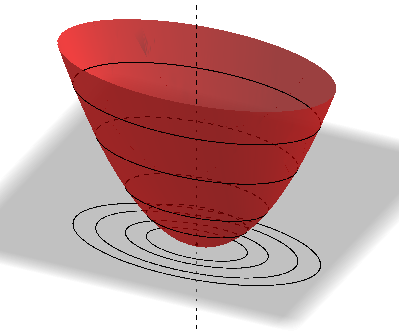
\includegraphics[width=0.4\textwidth]{elliptic-paraboloid-for-center.png}
  
    \caption{Центры эллипсов-сечений~---~на оси эллиптического параболоида.}
    \label{fig:elliptic-paraboloid-for-center}
  \end{figure}
  
  Если же поверхность~---~гиперболический параболоид, то сечения плоскостями $z \hm= c$, $c \hm\in \RR$ дают семейство концентрических гипербол~(\ref{fig:hyperbolic-paraboloid-for-center}).
  Их центры снова лежат на одной прямой.
  Которая проходит через седловую точку параболоида.
  Таким образом, снова координаты центра исходной кривой (гиперболы) можно искать из соотношения $\nabla \Phi(x_0, y_0) \hm= 0$.
  
  \begin{figure}[h]
    \centering

    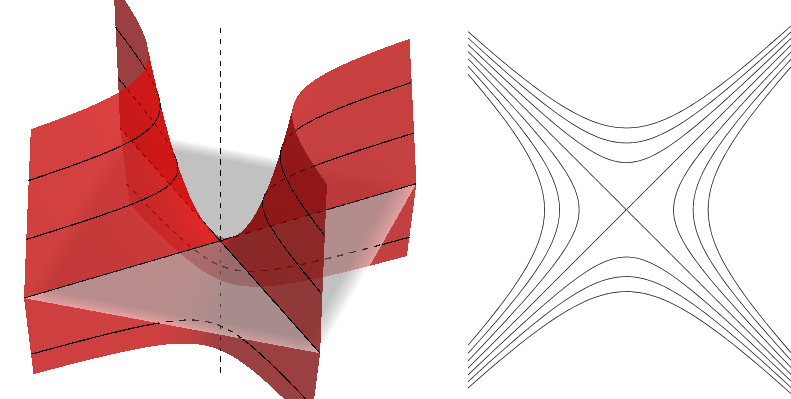
\includegraphics[width=0.8\textwidth]{hyperbolic-paraboloid-for-center.png}
  
    \caption{Центры гипербол-сечений~---~на той же оси, что и седловая точка гиперболического параболоида.}
    \label{fig:hyperbolic-paraboloid-for-center}
  \end{figure}
  
  
  \medskip
  
  \emph{Ещё один ``строгий'' вывод формул для поиска координат центра~---~но в матричном виде}\footnote{Идея вывода взята из \href{https://math.stackexchange.com/a/1287530/451127}{math.stackexchange.com/a/1287530/451127} (англ.).}.
  
  Уравнение кривой второго порядка
  \[
    Ax^2 + 2Bxy + Cy^2 + 2Dx + 2Ey + F = 0
  \]
  можно переписать в матричном виде.
  Для этого введём обозначения:
  \[
    \widetilde A \equiv \begin{pmatrix}
      A & B\\
      B & C
    \end{pmatrix}, \bds b \equiv \begin{pmatrix}
      D \\ E
    \end{pmatrix}, \bds x \equiv \begin{pmatrix}
      x \\ y
    \end{pmatrix}
  \]
  
  После этого уравнение кривой можно переписать следующим образом:
  \[
    \bds x \widetilde A \bds x^T + 2 \bds x \bds b^T + F = 0
  \]
  
  Если ввести обозначение $\bds \alpha \hm= (\alpha, \beta)^T$, то условие~(\ref{eq:center-definition}) на поиск координат центра $\bds x_0 \hm= (x_0, y_0)^T$ в матричном виде будет выглядет так:
  \[
    (\bds x_0 + \bds \alpha) \widetilde A (\bds x_0 + \bds \alpha)^T + 2 (\bds x_0 + \bds \alpha) \bds b^T + F
      = (\bds x_0 - \bds \alpha) \widetilde A \bds (\bds x_0 - \bds \alpha)^T + 2 \bds (\bds x_0 - \bds \alpha) \bds b^T + F
  \]
  
  Раскрывая скобки и упрощая, приходим к условию:
  \[
    \widetilde A \bds x_0 + \bds b = 0
  \]
  
  Иными словами (в скалярном виде):
  \[
    \left\{
      \begin{aligned}
        &Ax_0 + By_0 + D = 0\\
        &Bx_0 + Cy_0 + E = 0
      \end{aligned}
    \right.
  \]
\end{document}
